\chapter{Exercise 1}
The purpose of this exercise is to give a short introduction to
create, edit, link and run C/C++ programs that are based on the
graphics library OpenGL, and the utility libraries Angel and
GLUT.
\section{Part 1}
I drew another triangle by adding extra 3 vertices to the vertexData array:
\begin{figure}[ht!]
	\begin{center}
		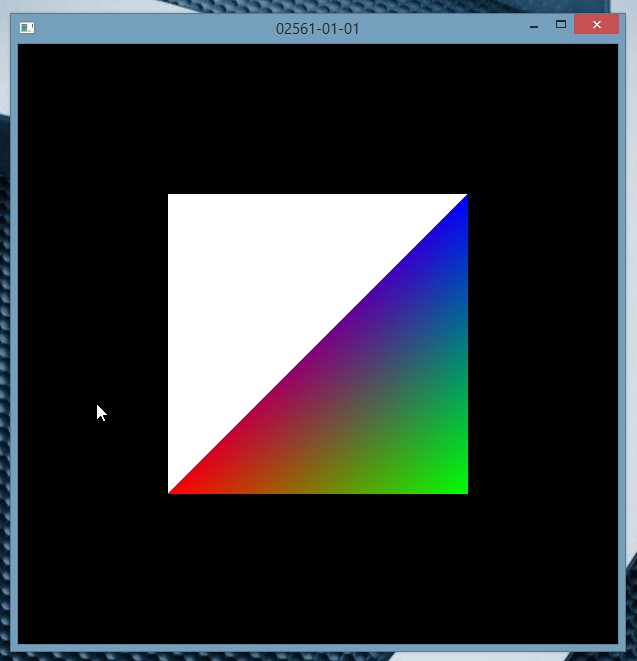
\includegraphics[width=0.5\textwidth]{figures/exercise_1_part_1}
	\end{center}
	\caption{Exercise 1 part 1 output}
\end{figure} \\
Below I described a meaning of each function used in a program:
\begin{description}
	\item[glGetAttribLocation] -- Returns the location of an attribute variable
	\item[glClearColor] -- specify clear values for the color buffers
	\item[glClear] -- clear buffers to preset values
	\item[glUseProgram] -- Installs a program object as part of current rendering state
	\item[glBindVertexArray] -- binds the vertex array object with name
	\item[glDrawArrays] -- render primitives from array data
	\item[glutSwapBuffers] -- swaps the buffers of the current window if double buffered
	\item[glViewport] -- sets the viewport
	\item[glGenVertexArrays] -- generate vertex array object names
	\item[glGenBuffers] -- generate buffer object names
	\item[glBindBuffer] -- bind a named buffer object
	\item[glBufferData] -- creates and initializes a buffer object's data store
	\item[glVertexAttribPointer] -- specify the location and data format of the array of generic vertex attributes at
	index index to use when rendering
	\item[Angel::InitShader] -- initializes shader programs stored in files passed as attributes
	\item[glutInit] -- initializes the GLUT library
	\item[glutInitContextVersion] -- sets openGL version we use
	\item[glutInitContextFlags] -- sets flags in GLUT library
	\item[glutInitContextProfile] -- sets profile of GLUT library
	\item[glutInitDisplayMode] -- sets the initial display mode
	\item[glutCreateWindow] -- creates a top-level window with a name passed as argument.
	\item[glutDisplayFunc] -- sets the display callback for the current window
	\item[glutReshapeFunc] -- sets the reshape callback for the current window
	\item[glutReshapeWindow] -- sets the window width and height
	\item[Angel::InitOpenGL] -- initializes OpenGL
	\item[glutMainLoop] -- enters the GLUT event processing loop
\end{description}
\section{Part 2}
I extended the program to include a triangle and rotated a rectangle using code below:
\begin{lstlisting}[language=cpp, caption={Exercise 1 part 1 code changes}]
void loadGeometry(){
// add a triangle
Vertex triangleData[triangleSize] = {
	{ vec2(2,2), vec3(1.0, 0.0, 0.0) },
	{ vec2(5,2), vec3(0.0, 1.0, 0.0) },
	{ vec2(3.5,5), vec3(0.0, 0.0, 1.0) }};
triangleVertexArrayBuffer = loadBufferData(triangleData, triangleSize);}

void display(){
// to rotate rectangle
mat4 modelView2 = Angel::RotateZ(45);
glUniformMatrix4fv(modelViewUniform, 1, GL_TRUE, modelView2);
// transform and render the triangle
mat4 modelView;
modelView[0][3]=6;
modelView[1][3]=7;
modelView[2][3]=0;
glUniformMatrix4fv(modelViewUniform, 1, GL_TRUE, modelView);
glBindVertexArray(triangleVertexArrayBuffer);
glDrawArrays(GL_TRIANGLE_FAN, 0, triangleSize);}
\end{lstlisting}
After applying these changes I got an output: \\
\begin{figure}[ht!]
	\begin{center}
		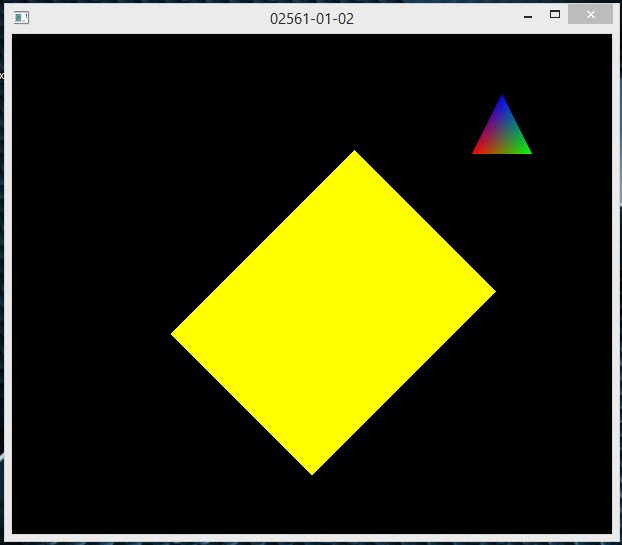
\includegraphics[width=0.45\textwidth]{figures/exercise_1_part_2}
	\end{center}
	\caption{Exercise 1 part 2 output}
\end{figure}